%******************************************************************************%
%                                                                              %
%                  html_css.en.tex for LaTeX                             %
%                  Created on : Tue Mar 10 13:27:28 2015                       %
%                  Made by : Dax Wann                                          %
%                                                                              %
%******************************************************************************%

\documentclass{42-en}

%******************************************************************************%
%                                                                              %
%                                    Header                                    %
%                                                                              %
%******************************************************************************%
\begin{document}
                           \title{Responsive Web Design}
                          \subtitle{With CSS Flexbox and CSS Grid}
                       \member{Dax Wann}{daxwann@gmail.com}
                        \member{42 Staff}{pedago@42.fr}

\summary {
  An introduction to designing responsive websites with HTML and CSS.
}

\maketitle

\tableofcontents


%******************************************************************************%
%                                                                              %
%                                  Foreword                                    %
%                                                                              %
%******************************************************************************%
\chapter{Foreword}

    \begin{figure}[H]
        \begin{center}
            
\includegraphics[width=12cm]{george-orwell.jpg}
        \end{center}
    \end{figure}
“You are a slow learner, Winston."\\
"How can I help it? How can I help but see what is in front of my eyes? Two and two are four."\\
"Sometimes, Winston. Sometimes they are five. Sometimes they are three. Sometimes they are all of them at once. You must try harder. It is not easy to become sane.”\\

- \textit{1984} by George Orwell
    
%******************************************************************************%
%                                                                              %
%                                 Introduction                                 %
%                                                                              %
%******************************************************************************%
\chapter{Introduction}

Now that you have completed a static website with basic HTML and CSS, we will continue with Responsive Web Design. \\


With the skills of using CSS Flexbox and Grid, you will be able to design websites that's responsive to the user's devices.



%******************************************************************************%
%                                                                              %
%                                  Goals                                       %
%                                                                              %
%******************************************************************************%
\chapter{Goals}

Using FreeCodeCamp online curriculum, we will learn:
\begin{itemize}
    \item Responsive web design principles
    \item CSS Flexbox
    \item CSS Grid
\end{itemize}

For our culminating project, we will apply what we learned to create a responsive gallery website similar to \href{https://www.pinterest.com/}{Pinterest}, where you share your interests through images of anything you like (but not offensive to others), like fashion, cars, technology, art, etc. We will push our project onto a Github repository and deploy our website with Github Pages to showcase.



%******************************************************************************%
%                                                                              %
%                             General instructions                             %
%                                                                              %
%******************************************************************************%
\chapter{General instructions}

\begin{enumerate}
    \item Make sure you can explain to your peers about how you built your responsive website using CSS Flexbox and/or Grid
    \item Reflect on what you learned in FreeCodeCamp and how you applied it to your project
\end{enumerate}
   
    



%******************************************************************************%
%                                                                              %
%                             Mandatory part                                   %
%                                                                              %
%******************************************************************************%
\chapter{Mandatory part}

You must have finished \texttt{Web Design with Basic HTML and CSS} project.\\

Finish all exercises in these following sections on FreeCodeCamp Responsive Web Design Certificate:
\begin{itemize}
    \item Responsive Web Design Principles
    \item CSS Flexbox
    \item CSS Grid
\end{itemize}
\vspace{0.2in}

Create a responsive gallery website using HTML5 and CSS Flexbox and/or Grid.\par
\vspace{0.2in}
Push your website project repository onto your Github. Deploy your website on github.io.
    


%******************************************************************************%
%                                                                              %
%                             Exercises of a Piscine                           %
%                                                                              %
%******************************************************************************%

\chapter{Exercise 00: Responsive Web Design Principles}

\extitle{Responsive Web Design Principles on FreeCodeCamp}
\exnumber{\exercicenumber}
\exscore{2}
\exfiles{All exercises completed in section on FreeCodeCamp}
\exauthorize{All}

\makeheaderfiles

Since users can view our website with different devices in various sizes, such as on a laptop, a gaming monitor, a mobile phone, or an iPad, we need to make our website adapt to the screen size. We use responsive web design to create different styles and layouts for different device sizes.

%******************************************************************************%
%                                                                              %
%                             Exercises of a Piscine                           %
%                                                                              %
%******************************************************************************%

\chapter{Exercise 01: CSS Flexbox}

\extitle{CSS Flexbox on FreeCodeCamp}
\exnumber{\exercicenumber}
\exscore{2}
\exfiles{All exercises completed in section on FreeCodeCamp}
\exauthorize{All}

\makeheaderfiles

CSS Flexbox is a new responsive layout feature that will help arrange elements within a parent container.\par
\vspace{.2in}
Learn more about CSS Flexbox here: \par
\url{https://css-tricks.com/snippets/css/a-guide-to-flexbox/}

%******************************************************************************%
%                                                                              %
%                             Exercises of a Piscine                           %
%                                                                              %
%******************************************************************************%

\chapter{Exercise 02: CSS Grid}

\extitle{CSS Grid on FreeCodeCamp}
\exnumber{\exercicenumber}
\exscore{2}
\exfiles{All exercises completed in section on FreeCodeCamp}
\exauthorize{All}

\makeheaderfiles

Similar to Flexbox, CSS Grid is another responsive layout feature that will help arrange elements within a parent container.\par
\vspace{.2in}
Learn more about CSS Grid here: \par
\url{https://css-tricks.com/snippets/css/complete-guide-grid/}

%******************************************************************************%
%                                                                              %
%                             Exercises of a Piscine                           %
%                                                                              %
%******************************************************************************%

\chapter{Exercise 03: Responsive Web Design Project}

\extitle{Responsive Web Design Project}
\exnumber{\exercicenumber}
\exscore{2}
\exfiles{Your project folder should include index.html, style.css, and image files in "assets/" subdirectory}
\exauthorize{All}

\makeheaderfiles

Create a responsive image gallery with a similar layout as \href{https://www.pinterest.com/}{Pinterest}. \par

\begin{figure}[H]
    \begin{center}
        \includegraphics[width=14cm]{pinterest-screenshot.png}\\
        desktop view
    \end{center}
\end{figure}

\begin{figure}[H]
    \begin{center}
        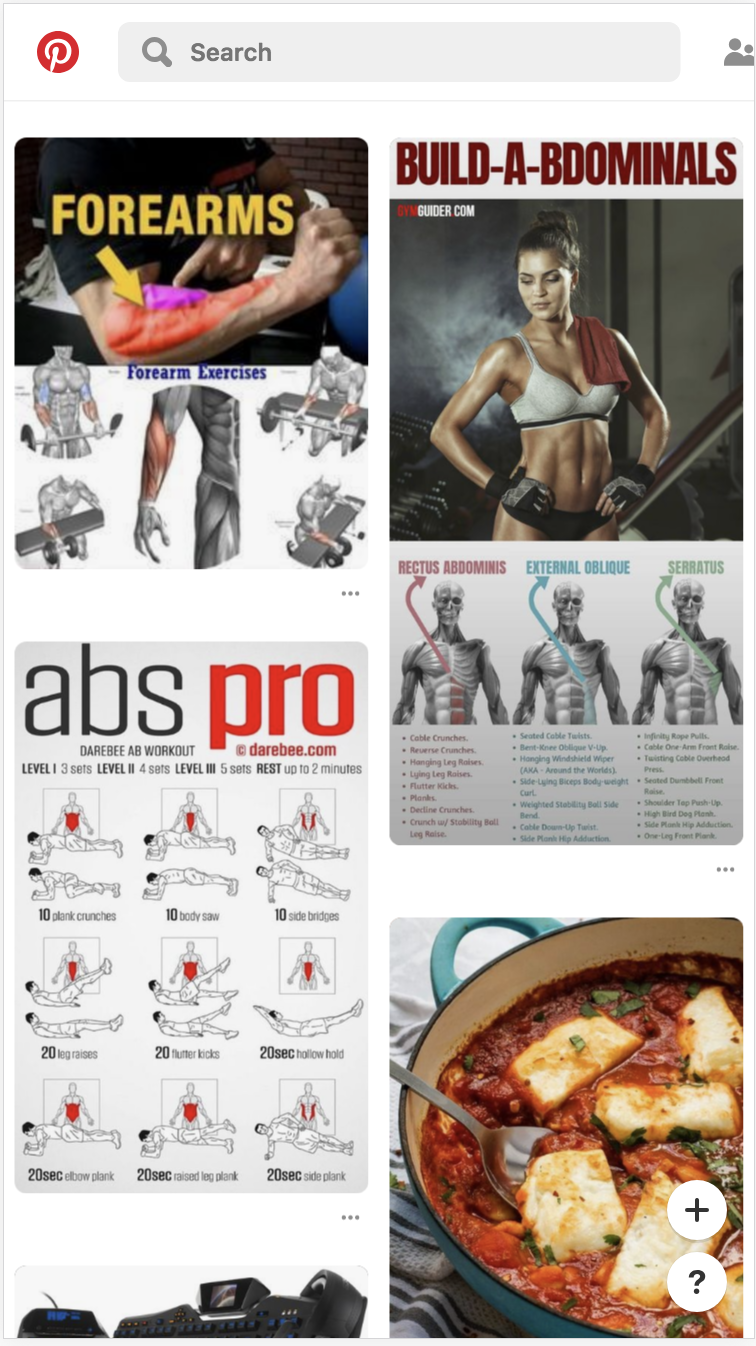
\includegraphics[width=5cm]{pinterest-mobile.png}\\
        mobile view
    \end{center}
\end{figure}

\vspace{.1in}
Requirements:
\begin{itemize}
    \item The page should have a fixed navbar that will stick to the top of the screen as you scroll down.
    \item The navbar should have the included Pinterest logo on the left side, and your first name on the right side.
    \item The main body of the gallery should have 20 or more images that represent your personal interests.
    \item The images should have the same width, but their individual height is adjusted according to the original image dimensions.
    \item There should be two images per row on mobile view.
    \item There should be between three to five images per row on ipad view.
    \item There should be six or more images per row on desktop view.
    \item Navbar should have display set to flex; Main gallery container should have display set to grid.
\end{itemize}
\vspace{.5in}
The final layout should be similar to the wireframes below
\begin{figure}[H]
    \begin{center}
        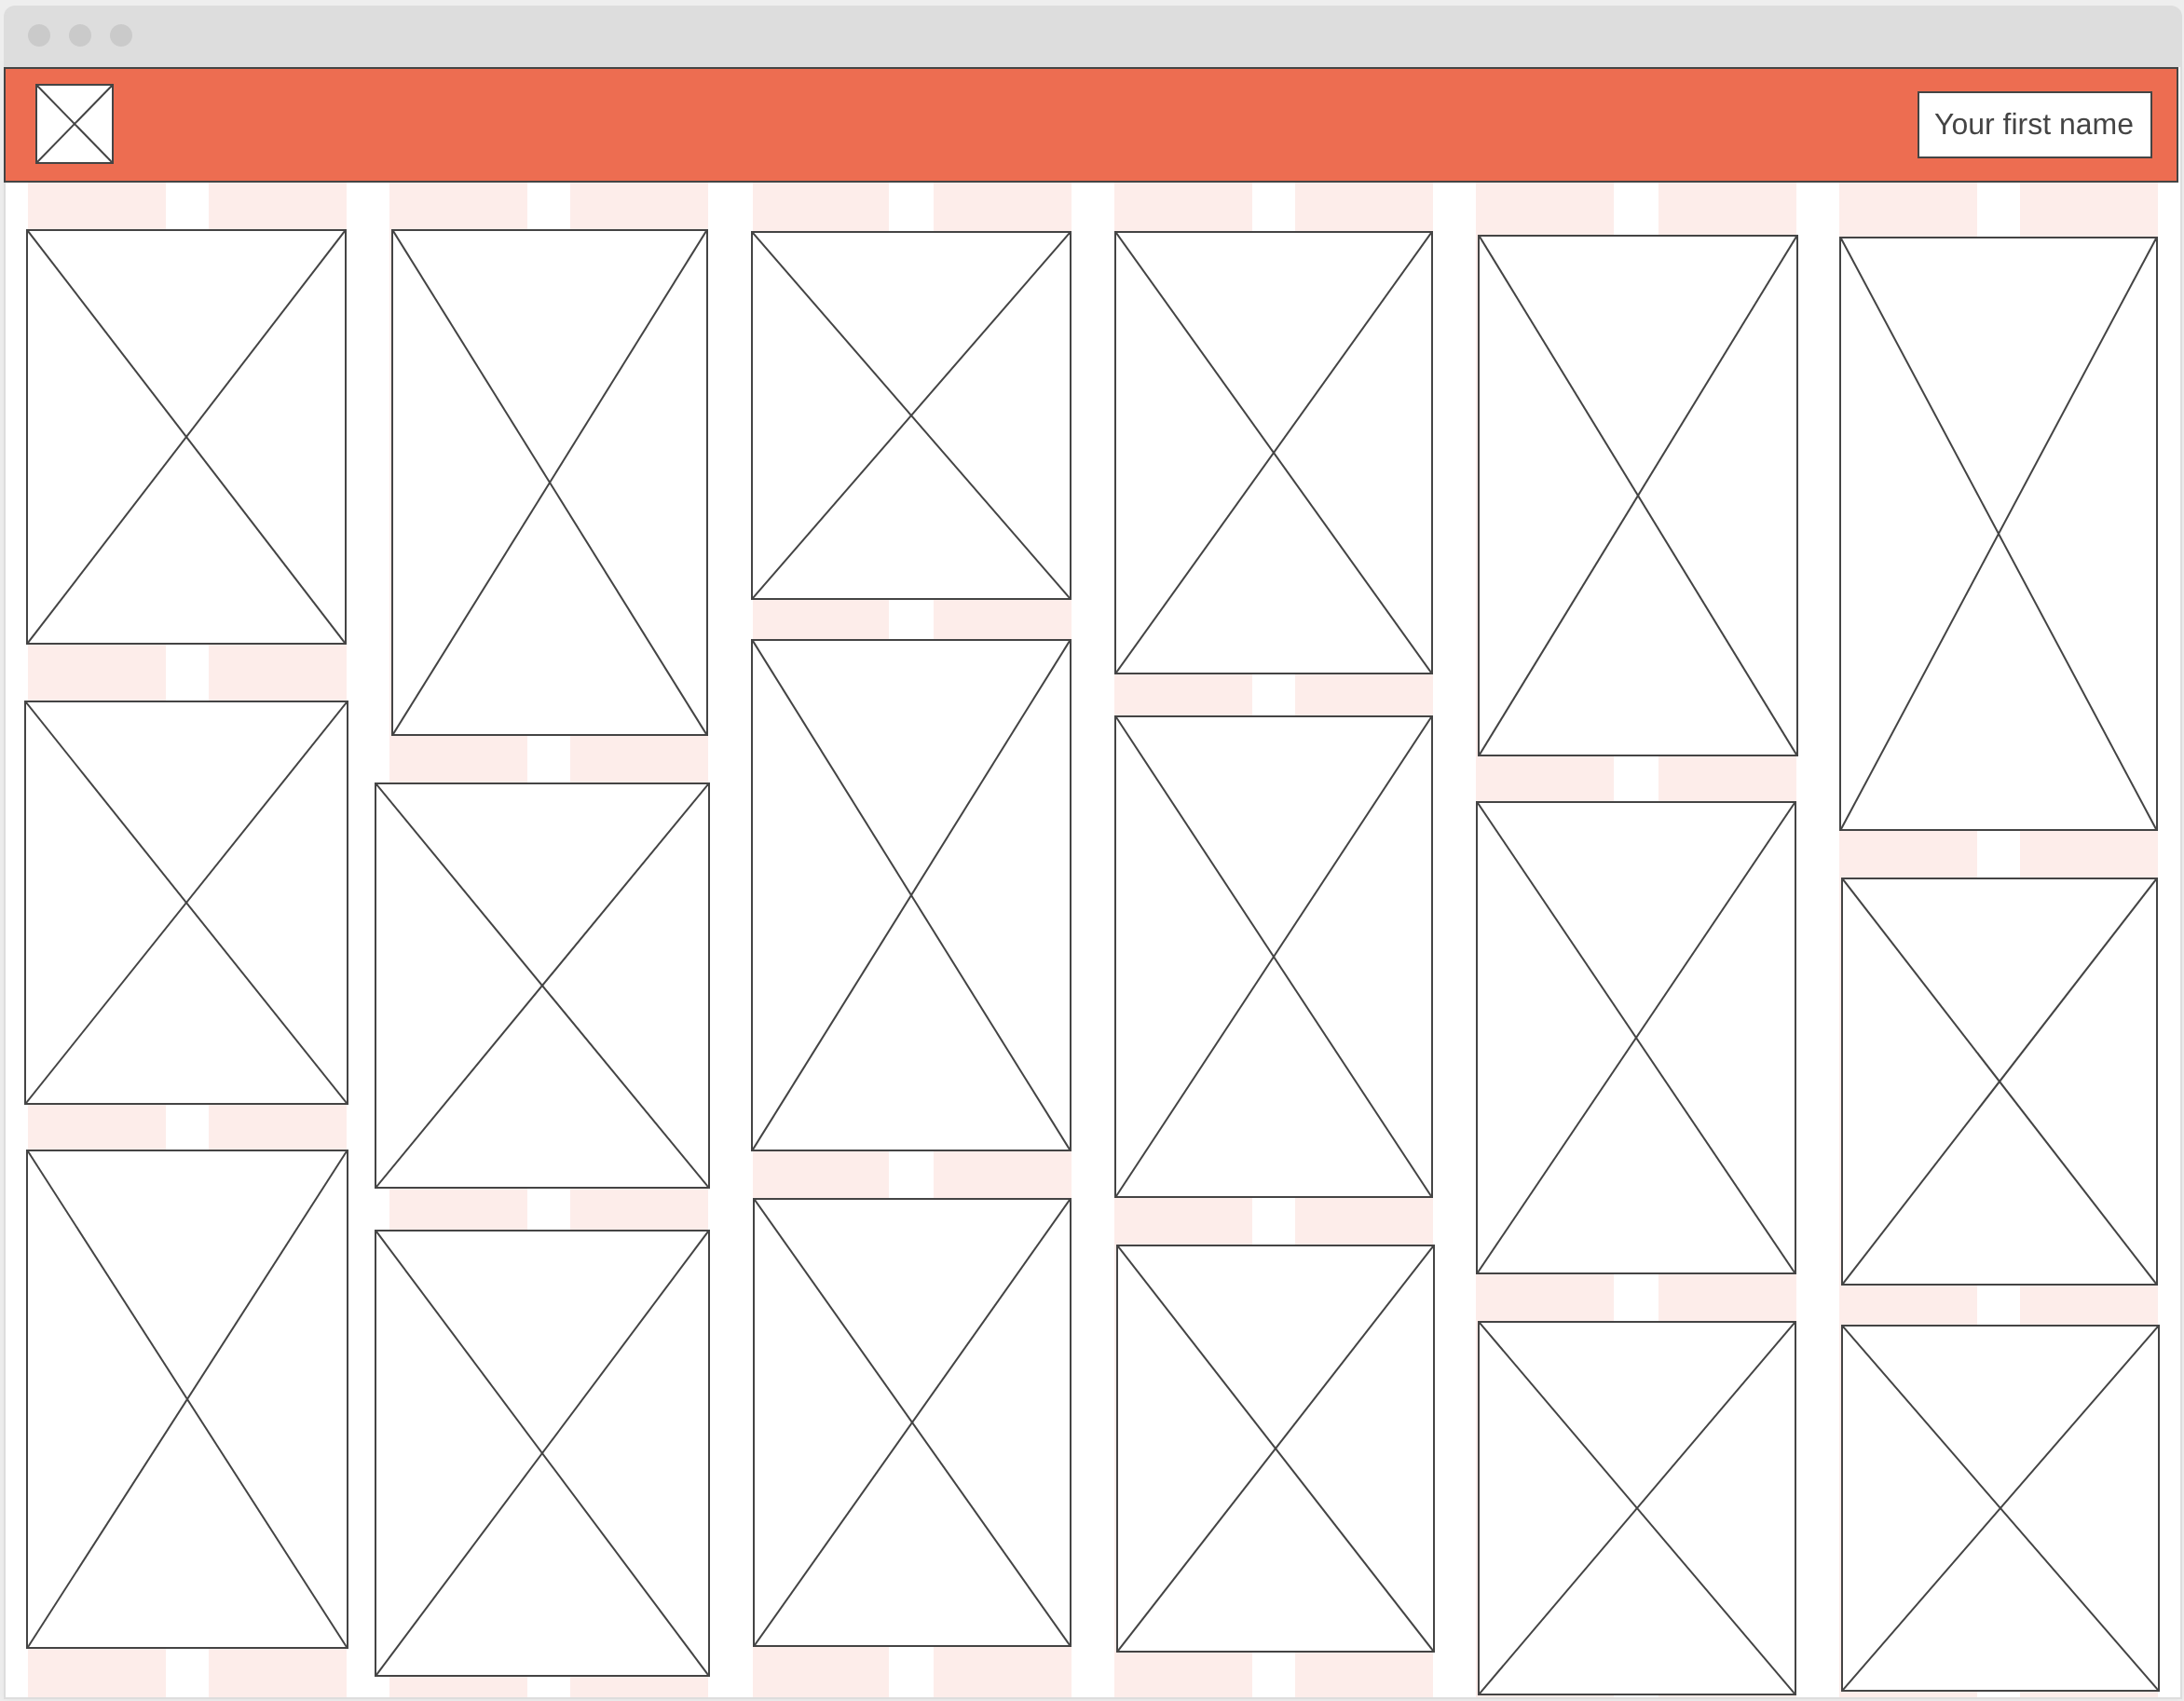
\includegraphics[width=12cm]{wireframe-desktop.png}\\
        desktop view
    \end{center}
\end{figure}
\begin{figure}[H]
        \begin{center}
            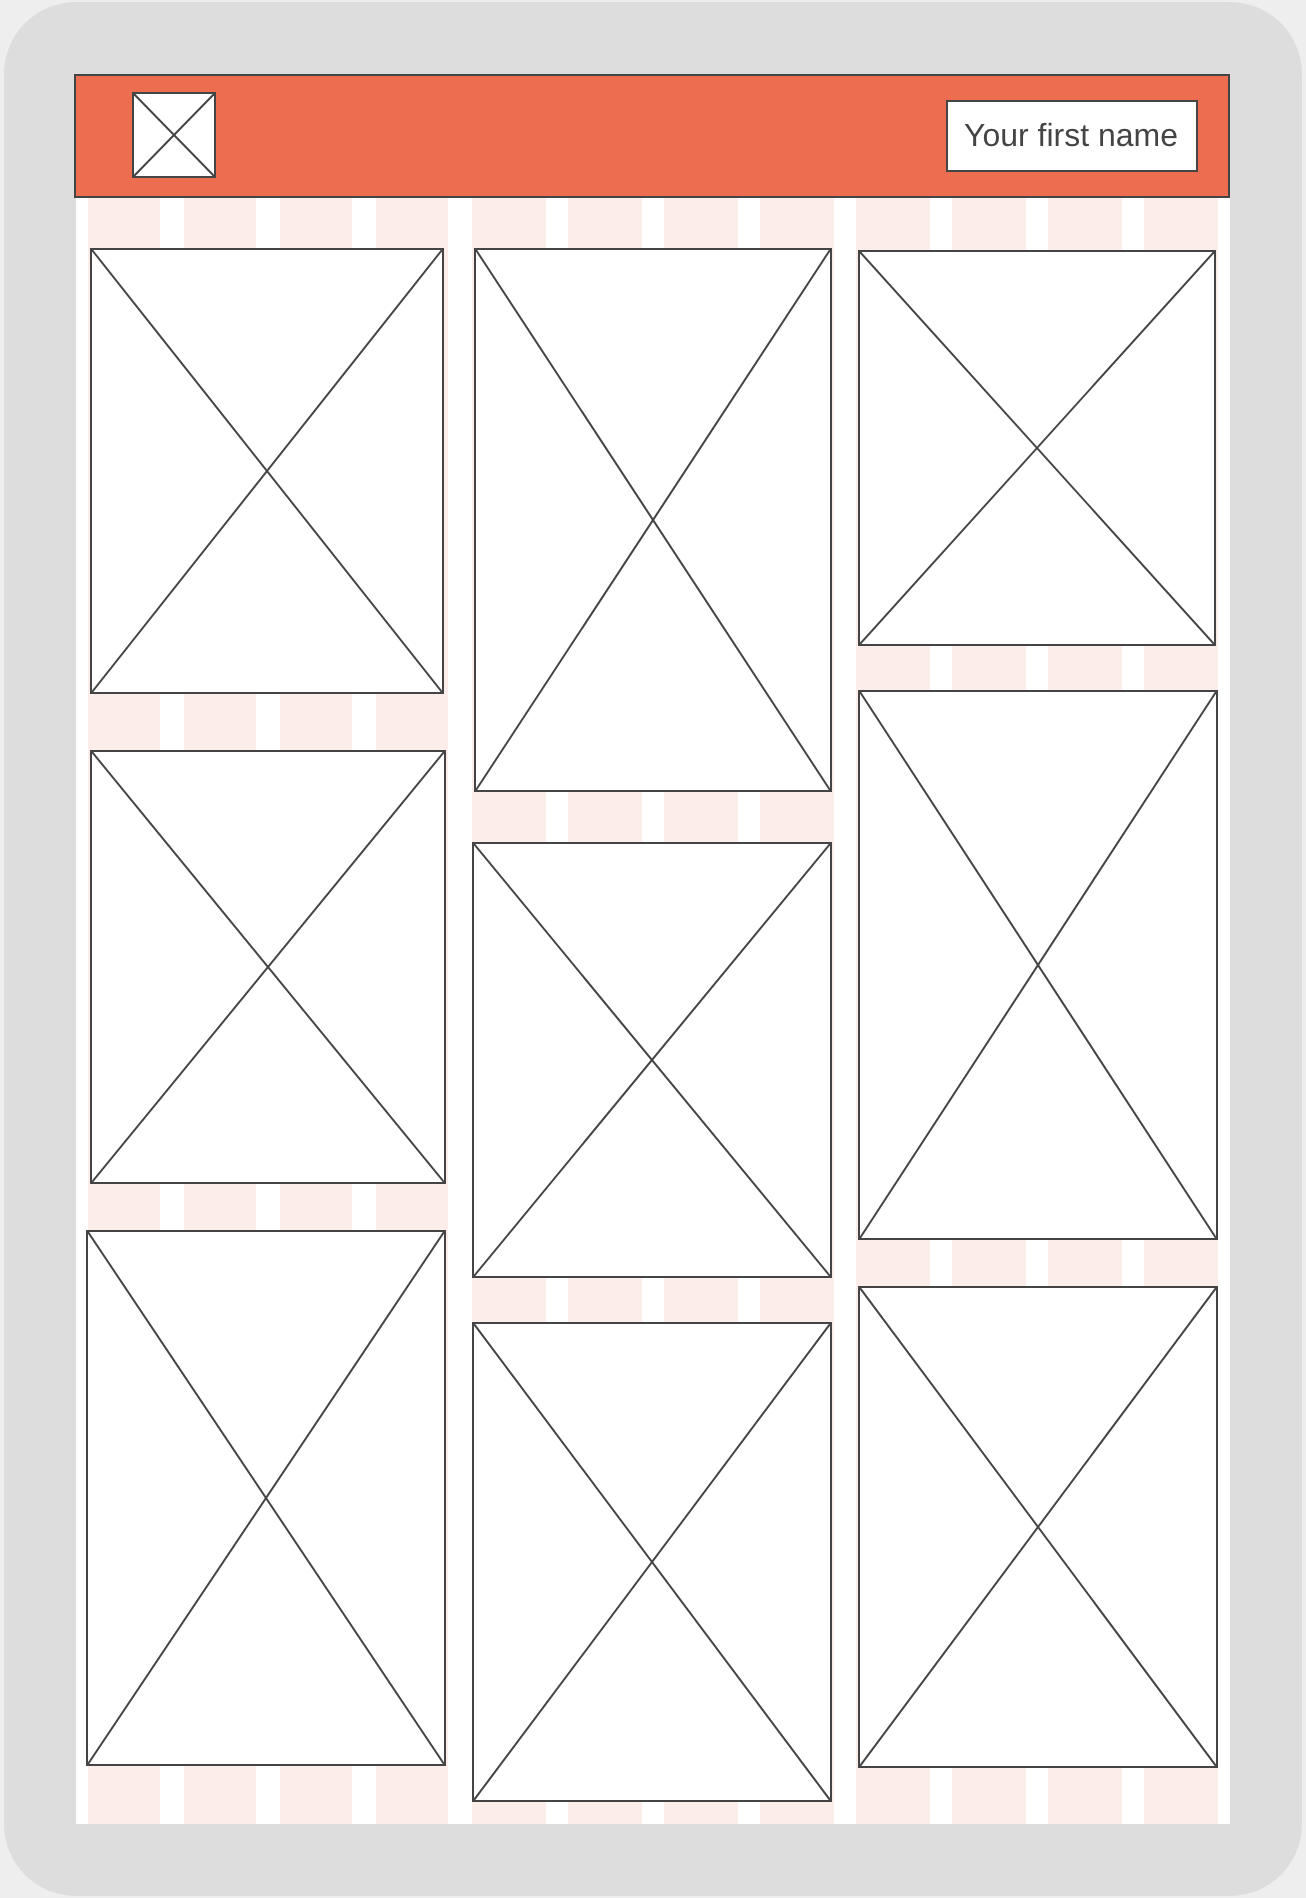
\includegraphics[width=8cm]{wireframe-ipad.png}\\
            ipad view
        \end{center}
\end{figure}
\begin{figure}[H]
        \begin{center}
            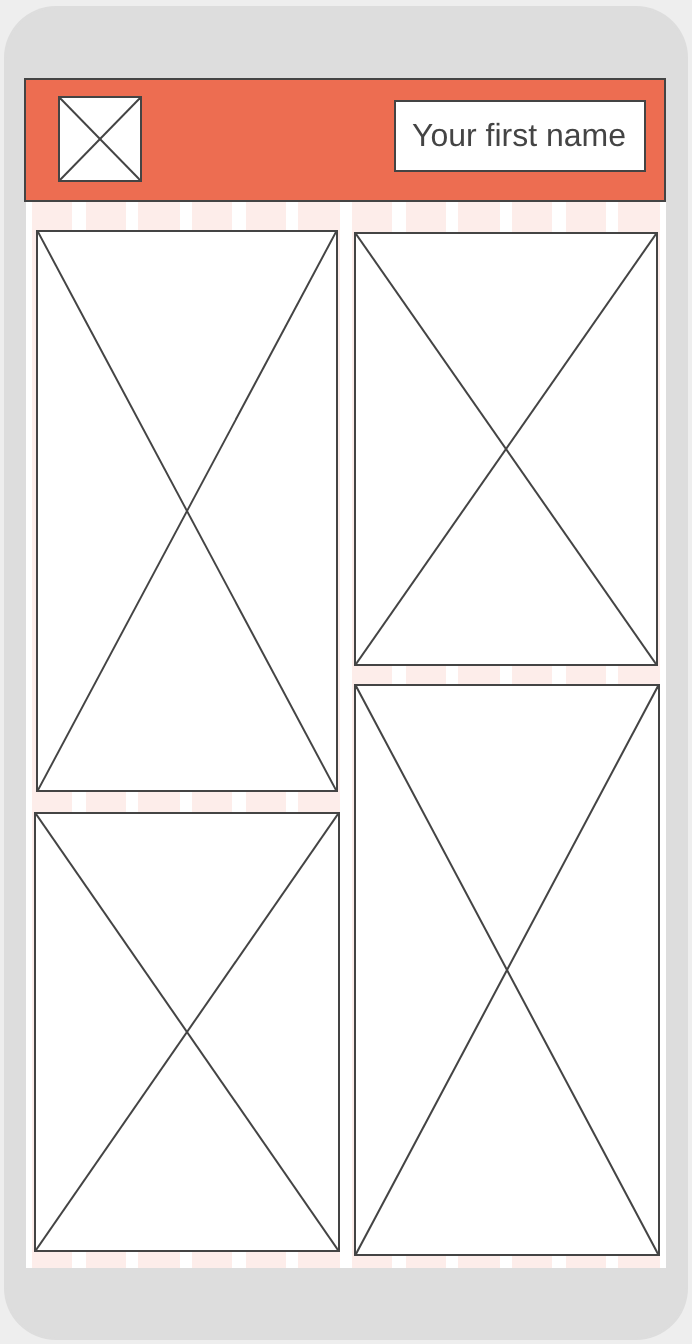
\includegraphics[width=4cm]{wireframe-mobile.png}\\
            mobile view
        \end{center}
    \end{figure}
    

\textbf{Suggestions}
\begin{enumerate}
    \item Create a project folder along with files \texttt{index.html} and \texttt{style.css}. Create a subfolder named \texttt{assets/} for images
    \item Use Visual Studio Code IDE to open the folder and start writing the HTML and CSS
    \item Apply what you learned in FreeCodeCamp to create the structure of the website and style it
    \item Use Chrome browser to test your website. You can access your website by opening the html file with Chrome or typing in its file path in the browser. If you are stuck, google first.
    \item Be sure to make the website responsive. Use \href{https://developers.google.com/web/tools/chrome-devtools/device-mode}{Chrome Developer Tools} to help you view your website on different devices.
\end{enumerate}

%******************************************************************************%
%                                                                              %
%                             Exercises of a Piscine                           %
%                                                                              %
%******************************************************************************%

\chapter{Exercise 04: Github}

\extitle{Deploy on Github}
\exnumber{\exercicenumber}
\exscore{2}
\exfiles{Your Github repository should include \texttt{index.html}, \texttt{style.css}, and image files in \texttt{assets/} subdirectory}
\exauthorize{All}

\makeheaderfiles

\begin{enumerate}
    \item You should already have a Github account.
    \item Create a new public repository named \texttt{H2S\_responsive\_gallery}
    \item Follow \href{https://help.github.com/en/articles/adding-a-remote}{instructions} on connecting your project to the new Github repository
    \item Push your project onto the Github repository
    \item Go to your Github repository settings, under "Github Pages", publish your project as a website. Follow the URL formatted as
    \begin{center}
        \texttt{<username>.github.io/H2S\_responsive\_gallery} \\
    \end{center}
    to view website.
    \item Create a \texttt{README.md} in the root directory of your project folder and copy the website URL into it. Follow this \href{https://help.github.com/en/articles/basic-writing-and-formatting-syntax#headings}{guide}.
\end{enumerate}

%******************************************************************************%
%                                                                              %
%                           Turn-in and peer-evaluation                        %
%                                                                              %
%******************************************************************************%
\chapter{Turn-in and peer-evaluation}

    Check that all exercises in the previously listed FreeCodeCamp sections have been completed.\\
    
    Check website is published on Github Pages.\\

    Turn your source code in using your \texttt{42 Git repository}. Only work present on your repository will be graded in defense.

%******************************************************************************%
\end{document}
